La gestione delle prenotazioni dei libri è una delle parte innovative introdotte dalla start up: questo servizio mira a sfruttare la flessibilità della community di sharing, basata sull'ideale di open-source, per comunque offrire un seervizio mirato ed attento alle necessità del lettore.
Ogni utente, purchè sia registrato all'interno del servizio di Book-sharing, può prenotare un determinato libro che si trova nello stato "Under reading".

Andiamo ad evidenziare gli attori coinvolti in questa operazione:
\begin{itemize}
	\item \textbf{\underline{Lettore} [L]:} esso rappresenta l'utente, registrato nella community, che possiede il libro oggetto della prenotazione. Indichiamo con:
	\begin{itemize}
		\item \textbf{{\LARGE $r_{L}$}:} raggio d'azione del lettore;
		\item \textbf{{\LARGE $ z_{0} $}:} zona di residenza (espressa come coordinate puntuali).
	\end{itemize}
	\item \textbf{\underline{Prenotanti} [$ P_{i}$ con $i=1,...,N $]:} rappresentano l'insieme degli utenti, tutti interessati ad uno specifico libro in possesso dell'utente \textbf{L}.
	Nello specifico l'indice \textit{i-esimo} indica l'ordine temporale con cui sono giunte le prenotazioni per lo specifico libro.
	Oltre a questa informazione, ogni utente, rappresentando un generico utente della community, avrà fornito, al momento della registrazione, le seguenti informazioni:
	\begin{itemize}
		\item \textbf{{\LARGE $r^{P}_{i}$} con $i=1,...,N $:} raggio d'azione del lettore;
		\item \textbf{{\LARGE $z^{P}_{i}$} con $i=1,...,N $:} zona di residenza.
	\end{itemize}

	L'algoritmo può essere scomposto in due macro-blocchi:
	\begin{itemize}
		\item \textbf{Step 0:} questo fase viene realizzata nel momento in cui il sistema inizia ad analizzare tutti gli utenti che hanno effettuato una prenotazione per un determinato libro che si trova nello stato di "Under reading".
		
		Tutti gli N prenotanti \textit{$ P_{i} $} vengono ordinati in base alla distanza dal lettore \textit{L}, indipendentemente da quello che è l'ordine temporale con cui è stata effettuata la prenotazione: la quantità di cui si terrà (come si può vedere nella figura ~\ref{fig:DistanceAlgorithm}) conto sarà quindi la distanza
		{\LARGE \begin{equation}
			|z^{p}_{i}-z_{0}|
		\end{equation}}
		\begin{figure}[h!]
		\centering
		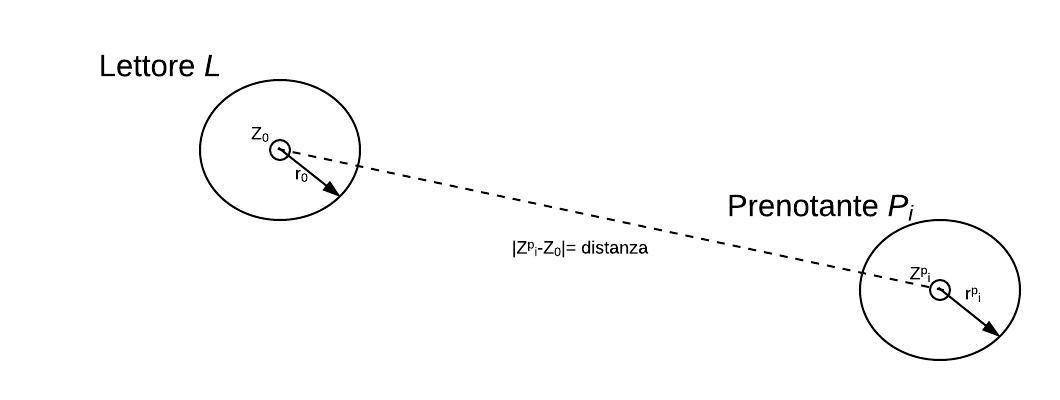
\includegraphics[width=0.8\textwidth]{Immagini/Algoritmo_Explanation}
		\caption{Distanza tra lettore e prenotante i-esimo}
		\label{fig:DistanceAlgorithm}
		\end{figure}
	
		Questo ordinamento corrisponde quindi sostanzialmente a creare una \textit{priority queue} in cui si va ad assegnare una maggiore priorità all'utente la cui zona di residenza è più vicina a quella del lettore in possesso del libro richiesto.
		
		\item \textbf{Step 1:} in questo macro-blocco andiamo effettivamente ad applicare l'algoritmo \textit{smart} per poter soddisfare, nella maniera migliore, le esigenze di ogni utente della community.
		
		
		L'idea di base è che, se lettore e prenotante hanno possibilità di incontrarsi, ovvero se i loro raggi d'azione si sovrappongono, essi potranno accordarsi direttamente sul luogo dello scambio, rendendo \textit{"safety"} il passaggio del libro: questo scambio avverrà ovviamente in una zona all'interno dell'intersezione dei raggi d'azione, come mostrato in figura ~\ref{fig:Zona_incontro}.
		
		\begin{figure}[h!]
			\centering
			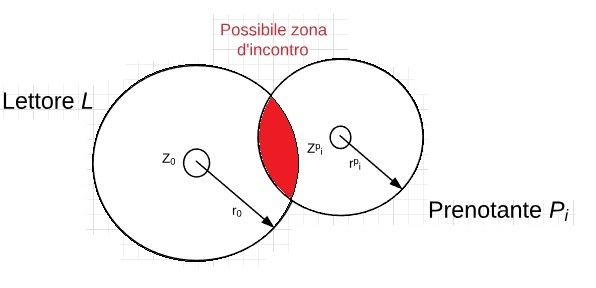
\includegraphics[width=0.6\textwidth]{Immagini/Algorithm_PuntoIncontro}
			\caption{Zona d'incontro tra lettore e prenotante}
			\label{fig:Zona_incontro}
		\end{figure}
	
		Nel caso in cui invece, i due utenti interessati non abbiano la possibilità di trovare un luogo comune in cui potersi scambiare il libro direttamente, si avrà che, la rete di users appartenenti alla community farà da tramite, per portare il libro \textit{"coast-to-coast"}.
		Quindi, tramite un semplice pseudo-codice, possiamo scrivere il nostro algoritmo come
	
		\begin{algorithm}[H]
			\SetAlgoLined
			\KwData{Users and their informations}
			\KwResult{Optimum path from reader to reserver}
			Step 0 (intilization)\;
			\eIf{Distanza <= 0}{
				Trova un punto d'incontro nell'unione delle delle area;
				
				Notifica gli utenti di dove potersi scambiare direttamente il libro;
			}{
				Crea la rete di utenti che faranno da tramite tra lettore e prenotante;
				
				Ricercare il cammino ottimo (il libro si muoverà \textit{hand-to-hand});
			}
			\caption{Algoritmo di gestione della prenotazione}
		\end{algorithm}
		
		
		Nello specifico il calcolo della distanza avverrà tramite la funzionalità \textit{VerificaPuntoIncontro(Lettore, Prenotante)} (TODO: inseire funzione effettiva), la quale andrà a verificare che:
		
		{\LARGE \begin{equation}
			|z^{p}_{i}-z_{0}|-r_{0}-r_{i}<=0
		\end{equation}}
		
		ovvero che i raggi d'azione si sovrappongano o meno.
		
		Nel caso in cui i due utenti non abbiano possibili punti d'incontro (Distanza $>= 0 $), dobbiamo selezionare gli utenti tramite il quale il libro in questione potrà viaggiare: l'idea base è quindi quella di costruirsi un'area circolare di centro pari alla metà della congiungente del punto $ z_{0} $ (zona di residenza lettore) e $ z^{p}_{i} $ (zona di residenza prenotante).
		Andremo poi a selezionare tutti gli utenti che si trovano all'interno di questa circoscrizione.
		In passi sequenziali, possiamo scrivere:
		
		\begin{algorithm}[H]
			\SetAlgoLined
			\KwData{Zona di residenza e raggio d'azione di utente lettore e prenotante}
			\KwResult{Elenco di utenti attraverso cui il libro dovrà spostarsi \textit{hand-to-hand}}
			
			
			Il raggio della circoscrizione di utenti coinvolti sarà pari alla distanza
			\[ \bar{Z} = \dfrac{1}{2} |z^{p}_{i}-z_{0}| \]
			\For{Tutti gli utwnti $ z_{i}^U $ nella community}{
			\If{$ (Distanza(z_{0},z_{i}^U)) <= \bar{Z} $ oppure $ (Distanza(z_{i}^P,z_{i}^U)) <= \bar{Z} $  }{
				
				Seleziono l'utente $ z_{i}^U $ e lo inserisco nella lista (\textit{HandToHandUsers}) dei possibili utenti che potrebbero partecipare attivamente al prestito;
			}
			}
			Creiamo il collegamento tra gli users della lista \textit{HandToHandUsers} il cui raggio d'azione si sovrappone\;
			\caption{Creazione del percorso tra lettore e prenotante}
		\end{algorithm}
		
		Quindi, alla fine dello step 1, avremo individuato tutti gli utenti i quali potrebbero partecipare attivamente alla realizzazione di un prestito: il risultato ottenuto sarà quindi come quello in figura ~\ref{fig:UsersNet}.
						
		\begin{figure}[h!]
			\centering
			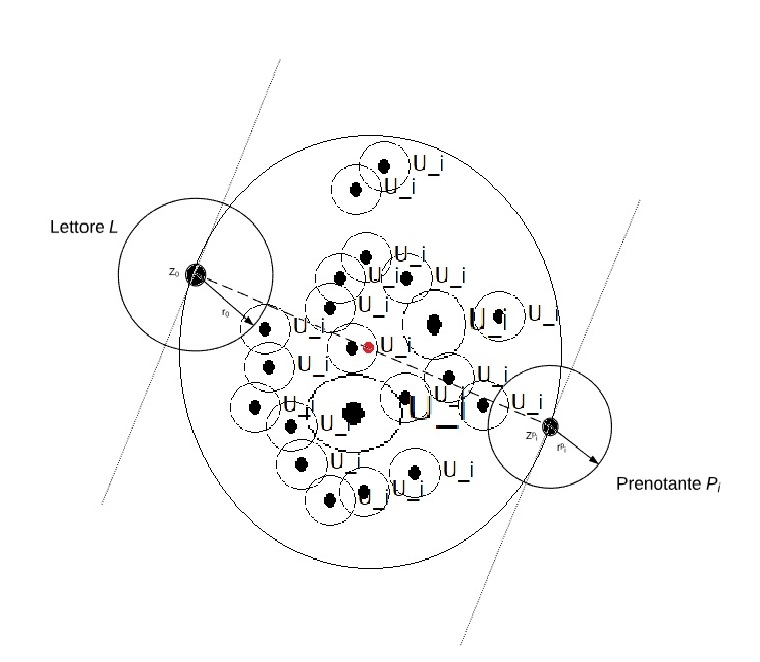
\includegraphics[width=0.8\textwidth]{Immagini/Algorithm_UsersNet}
			\caption{Rete di utenti che potrebbero essere attivi nel prestito}
			\label{fig:UsersNet}
		\end{figure}
		
	\end{itemize}
\end{itemize}

//TODO: move this comment to documentation

// Insieme di candidati: users == overlapping users
// Funzione obbiettivo: minimizzare i km che il libro deve fare / minimizzare il numero di utenti tra cui fare
// il passamano --> la scelgo in maniera epsilon - greedy


// Epsilon for epsilon greedy algorithm: during the path calculation for the reservation
// we choose usually the next user, as the nearest one.
// Using the greedy algorithm, with a probability that depends on the epsilon variable value, we choose the user
// with the biggest radius.
// epsilon lower --> algorithm stronger (always foound path to me)
// epsilon higher --> algorithm found sorthest path